\documentclass{article}
\usepackage[margin=1in]{geometry}
\usepackage{amsmath}
\usepackage{graphicx}
\usepackage{hyperref}
\usepackage{url}
\usepackage{fancyvrb}
\usepackage{listings}

\begin{document}
\title{Zumy Tutorial (cont'd)}
\author{James Lam Yi}
\date{\today}
\maketitle
This document provides an instruction to control multiple Zumies for navigation and network discovery in a ROS environment, and this document is based on completion of previous Zumy tutorial. We provide examples for using \verb=RQT robot steering=\footnote{\url{http://wiki.ros.org/rqt_robot_steering}} and \verb=Man Joy Override=\footnote{\url{https://github.com/jlamyi/man_joy_override}} package for driving multiple Zumies. 

\section{Setup}
\subsection{Auto Connect}
\verb=Auto Connect= is a ROS node in \verb=odroid machine= package that allows the host automatically awakes Zumies as soon as they are connected to local network. This node detects new Zumy connections via \verb=Avahi=\footnote{\url{http://www.avahi.org/}}, displays lists of different status for detected Zumies, and tries to awake and reconnect these Zumies. 

In this node, detected Zumies are divided into three lists of different status: \verb=online=, \verb=alive= and \verb=lost=.  On the status of \verb=online=, Zumies are detected by the host via local network, but the host fails to receive ROS hearts beat from them. On this status, the host tries to awake Zumies to \verb=alive= status as soon as it receive ROS heart beat from the Zumy. On the status of \verb=alive=, Zumies are connected to local network, and the host receives ROS heart beats from them. Zumies in this status have established a good ROS connection with the host. On the status of \verb=lost=, Zumies are connected to local network once but currently lose connections. The host tries to search for these lost Zumies, and change their status to \verb=online= as soon as they are reconnected to the host.

Following steps are setup and tests for launching \verb=Auto Connect=:
 
\begin{enumerate}
\item Install dependencies
\begin{Verbatim}[frame=single]
sudo apt-get install nmap python-nmap
\end{Verbatim}

\item Download the package to the \verb=src= directory of a ROS workspace with
\begin{Verbatim}[frame=single]
git clone https://github.com/jlamyi/odroid_machine.git
\end{Verbatim}
and run \verb=catkin_make= from the workspace. If you have downloaded and installed \verb=Odroid machine=, skip this step.
 
\item Launch \verb=Auto Connect= with 
\begin{Verbatim}[frame=single]
roslaunch odroid_machine auto_connect.launch 
\end{Verbatim}

If it is successfully launched, the terminal repeatly shows "Online Detector: scanning...".

If the host connects to a Zumy successfully, the wheels of the Zumy will move a little bit. Also, terminal should output "... done launching nodes", but it is probably hard to be seen since there are too many terminal outputs for launching \verb=Auto Connect=.

\item To confirm if a Zumy has a solid ROS connection with the host, \verb=Auto Connect= provides lists for tracking Zumies status. Simply check out topic \verb=/online_detector/alive_robots= for \verb=alive= Zumies. If the host name of a Zumy is in the list of this topic, this Zumy has set up a solid ROS connection. Also, you can check out \verb=/online_detector/online_robots= and  \verb=/online_detector/lost_robots= for Zumies on status of \verb=online= and \verb=lost=.

\item If it hangs with terminal output "waiting for connection...", no Zumy is detected by the host. In this case, it waits until the first Zumy is detected by the host. If it waits for too long for connections, relaunch \verb=Auto Connect=.

\item If a Zumy fails to connect to the host, first, test its local network connection with
\begin{Verbatim}[frame=single]
ping "host name of the failed Zumy".local
\end{Verbatim} 

If terminal shows
\begin{Verbatim}[frame=single]
ping: unknown host "the host name of the failed Zumy"
\end{Verbatim} 
Restart the Zumy, and test its local network connection again with the command shown above.

\end{enumerate}

Also, \verb=rqt_graph=\footnote{\url{http://wiki.ros.org/rqt_graph}} should display Figure \ref{fig:auto_connect} , which shows that \verb=Auto Connect= is subscribing topic from \verb=Avahi= for new connection detection, and subscribing Zumy \verb=heart beat= to identify \verb=alive= Zumies. Then it publishes lists of \verb=online=, \verb=alive= and \verb=lost= status. 
\begin{figure}[h]
\centering
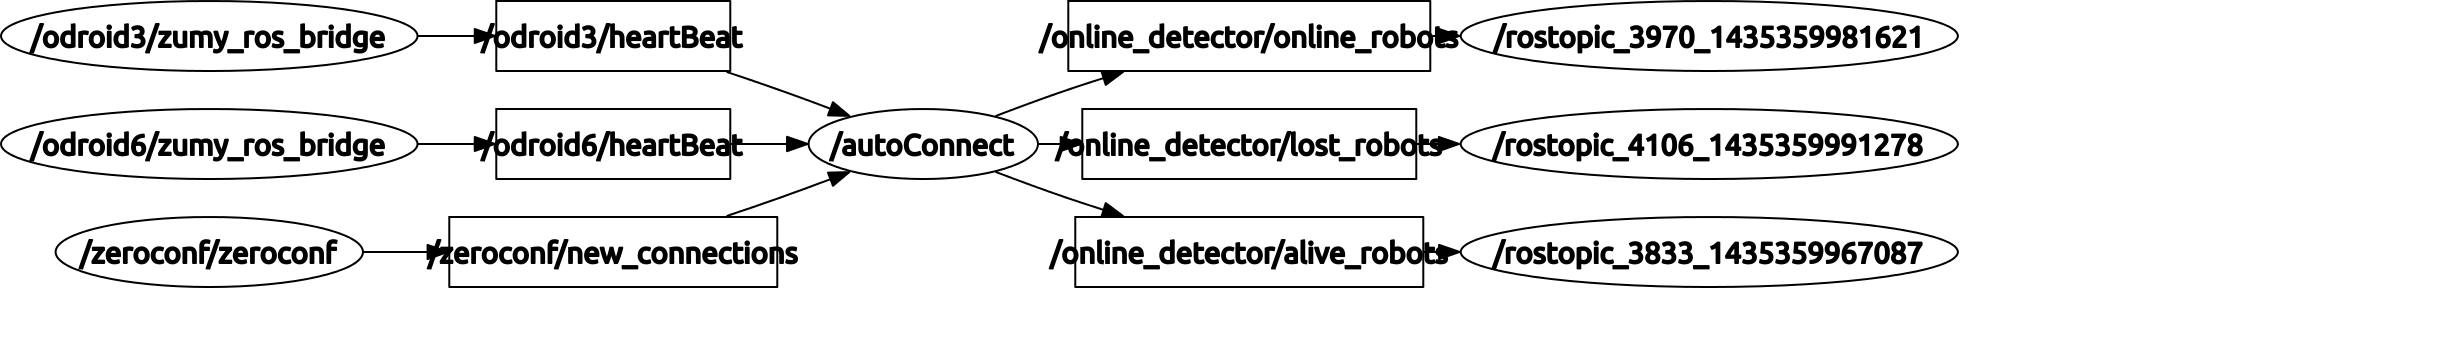
\includegraphics[width=1.3\textwidth]{img/auto_connect.png}
\caption{ROS node graph of Auto Connect}
\label{fig:auto_connect}
\end{figure}


\section{Drive}
\subsection{RQT robot steering}

Similar to previous turtorial, \verb=RQT robot steering= can be used to drive Zumies by publishing topics to them. Once a Zumy establishes a good ROS connection with the host, run \verb=RQT robot steering= with

\begin{Verbatim}[frame=single]
rosrun rqt_robot_steering rqt_robot_steering
\end{Verbatim} 
Modify pubilish topic name with the Zumy you want to drive, and modify the namespace of this topic if you want to drive other Zumies that are connected to the host. For example, to drive Zumy "zumy3", modify your topic to 

\begin{Verbatim}[frame=single]
/zumy3/cmd_vel
\end{Verbatim}

\begin{figure}[h]
\centering
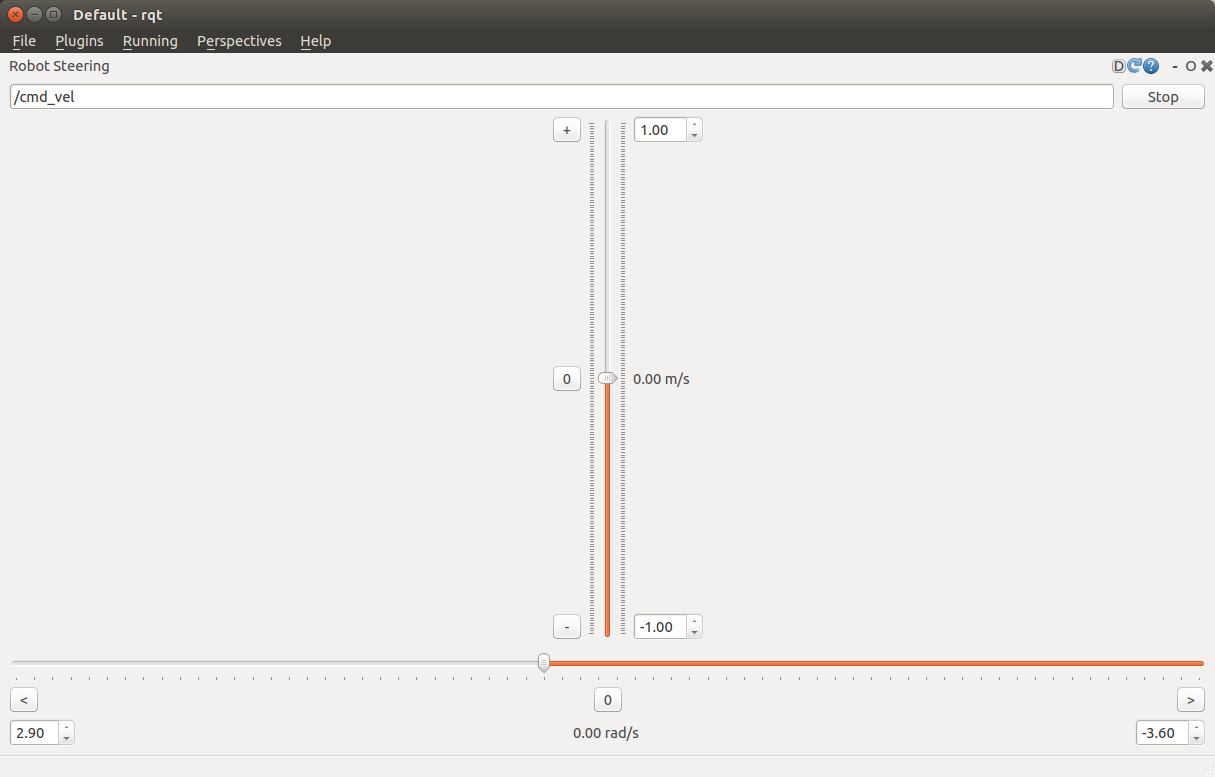
\includegraphics[width=0.7\textwidth]{img/rqt_robot_steering.png}
\caption{RQT robot steering plugin GUI}
\label{fig:robot_steering}
\end{figure}


\subsection{Man Joy Override}
\verb=Man Joy Override= is a ROS package developed in Fearing Biomimetics Millisystem Laboratory to allow manual override of commanded velocities with joysticks. It contains a multiplexer so that the user can switch to control different Zumies with the same joystick (currently it supports up to four Zumies with one joystick). 

Figure \ref{fig:mjo} shows the software architecture of \verb=Man Joy Override=. It reads joystick input by subscribing topic \verb=Joy=, and decides to which Zumy the host should send commands by subscribing topic \verb=/online_detector/alive_robot=.

\begin{figure}[h]
\centering
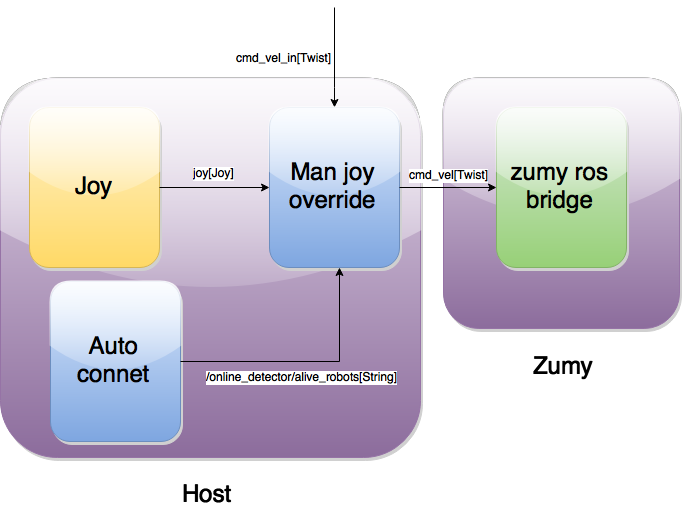
\includegraphics[width=0.6\textwidth]{img/ZumyROS.png}
\caption{Diagram of using Man Joy Override for driving Zumy}
\label{fig:mjo}
\end{figure}

This package can be downloaded with this command

\begin{Verbatim}[frame=single]
git clone https://github.com/jlamyi/man_joy_override.git
\end{Verbatim}

When the download is finished, compile the package from the workspace by running \verb=catkin_make=. After it is compiled, first, plug in \verb=Logitech Rumble Gamepad F510=\footnote{\url{http://support.logitech.com/product/rumble-gamepad-f510}} driver to the host (This type of driver was used for Zumy development in the lab). Then, launch \verb=Man Joy Override= with the command shown below (This launch file includes \verb=Auto Connect= and \verb=Joy= node. This should be the only command typed in terminal, and you should not seperately launch \verb=Auto Connect=).

\begin{Verbatim}[frame=single]
roslaunch man joy override zumy.launch 
\end{Verbatim} 

If you successfully launch \verb=Man Joy Override=, \verb=rqt_graph= should display the graph similar to Figure \ref{fig:man_joy_override}. \verb=Man Joy Override= subscribes topic \verb=joy= and \verb=/online_detector/alive_robots= from \verb=Joy= and \verb=Auto Connect=. It publishes velocity commands to Zumies while \verb=Auto Connect= subscribes \verb=heart beat= from Zumies.    

\begin{figure}[h]
\centering
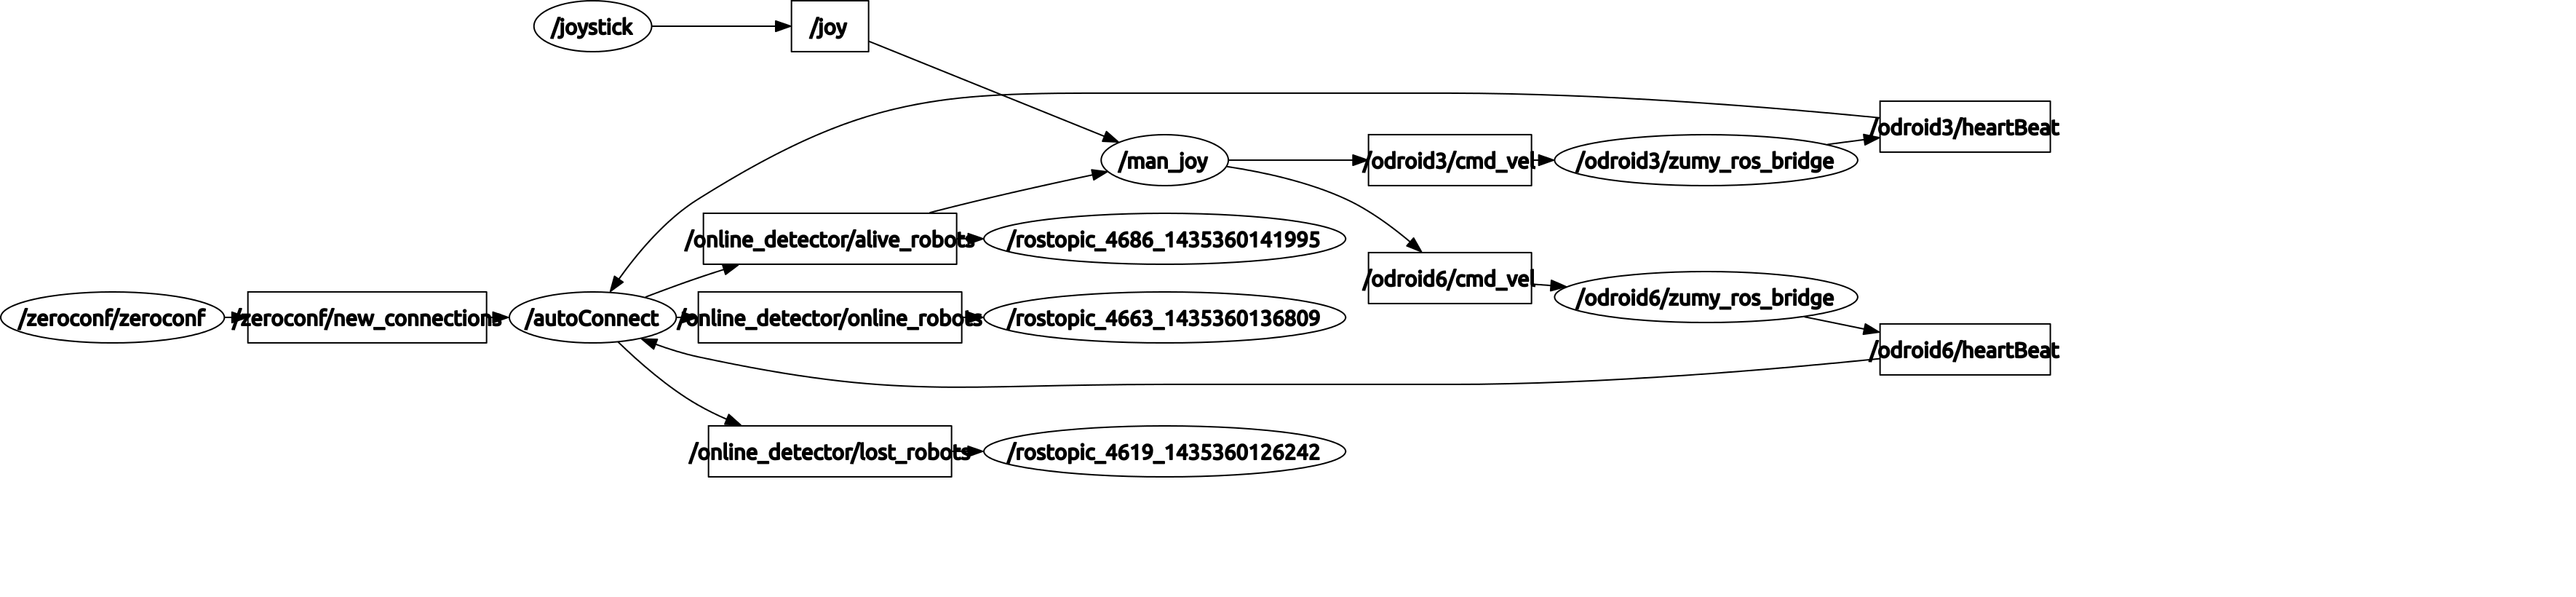
\includegraphics[width=1.3\textwidth]{img/man_joy_override.png}
\caption{ROS node graph of Man Joy Override}
\label{fig:man_joy_override}
\end{figure}

Figure \ref{fig:joy} shows a picture of \verb=Logitech Rumble Gamepad F510= driver. 

In \verb=Man Joy Override=, at most four Zumies can be controlled with one joystick, and the four colored buttons on the right map to four different Zumies. Start with the blue button, these buttons are clockwisely mapped to robot 0, 1, 2 and 3. The mapping relationship can be found in topic \verb=/online_detector/alive_robot=. The first four Zumies on this list are mapped to robot 0, 1, 2 and 3. 

To select a Zumy, you need to press the button mapped to the Zumy before driving it. The joystick on the right is the only joystick needed to drive a Zumy. Moving it up and down allows to drive a Zumy forward and backward, and moving it left and right allows to turn a Zumy left and right.   

\begin{figure}[h]
\centering
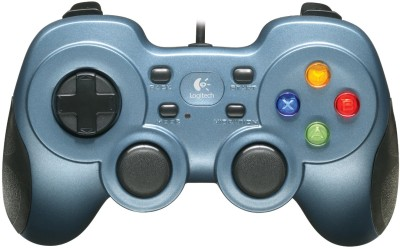
\includegraphics[width=0.5\textwidth]{img/joystick.jpeg}
\caption{Logitech Rumble Gamepad F510 driver}
\label{fig:joy}
\end{figure}


\end{document}
